
\chapter{Конструкторская часть}\label{Konstruct}
%\addcontentsline{toc}{chapter}{2 Конструкторская часть}

В данном разделе представлены схемы алгоритмов. Так же будут описаны пользовательские структуры данных, 
приведены классы эквивалентности для тестирования реализуемого ПО.

\section{Схема алгоритмов}\label{SchemaAlg}

На рисунке \ref{ris:schemaposav} показана схема алгоритмов работы диспетчера и каменщиков.

\begin{figure}[H]
  \center{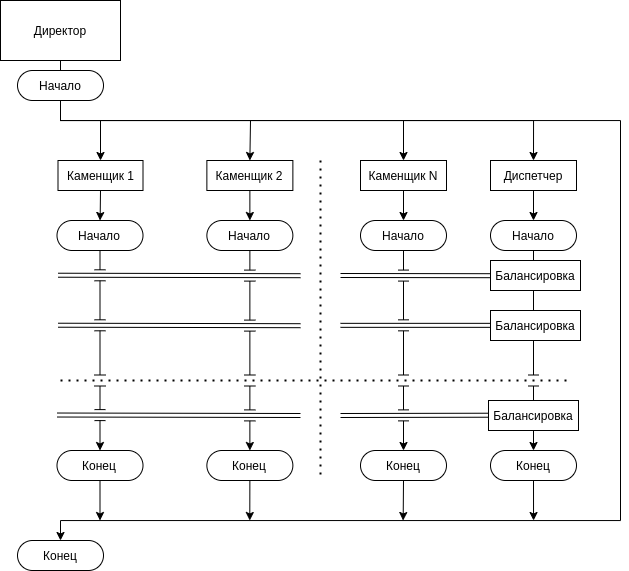
\includegraphics[scale=0.40]{l1.res}}
  \caption{Схема алгоритма полного перебора}
  \label{ris:schemaposav}
\end{figure}

\section{Структуры данных}\label{Structs}

При реализации приведенных алгоритмов потребуются типы данных: матрица кирпичей, кирпич, параметры системы.

Кирпич:

\begin{enumerate}
  \item название строителя 
  \item значение bool - установлен, или нет
\end{enumerate}

Параметры:

\begin{enumerate}
  \item ширина стены;
  \item высота стены;
  \item стартовая очередь кирпичей; 
  \item количество каменщиков;
  \item границы участков каждого каменщика;
  \item массив значений, где i - ое значение - количество установленных каменщиком.
\end{enumerate}
%\subsection{Способы тестирования}\label{TestingMethods}

%При разработке программы удобно использовать следующие методы тестирования:

%\begin{enumerate}
%    \item Модульные тесты 
%    \item Функциональные тесты 
%\end{enumerate}

\section{Вывод конструкторской части}\label{KonstructResult}

На основе данных, полученных в аналитическом разделе, была построена схема используемого алгоритма,
выделены необходимые для реализации структуры данных.

